\chapter{\IfLanguageName{dutch}{Resultaten}{Resultaten}}
\label{ch:resultaten}
\section{\IfLanguageName{dutch}{Bespreking requirementanalyse}{Analyzing requirementanalyse}}
De requirementanalyse heeft een beperkte steekproefomvang (n=70). Dit is echter niet problematisch, aangezien de opzet van de analyse niet is om te generaliseren naar de algemene populatie. Alleen water- en wintersporters werden bevraagd, dit is geen eenvoudige doelgroep om te bereiken. Bovendien werd de dataverzameling bemoeilijkt door de coronapandemie. Het was bijvoorbeeld niet mogelijk om respondenten te rekruteren op andere manieren dan via een online survey. De resultaten beperken zich tot een univariate bespreking. Meer complexe analyses behoren immers niet tot de reikwijdte van het onderzoek. Bovendien zouden de resultaten wellicht vertekend zijn door de beperkte steekproefomvang. Uit de analyse blijkt dat de overgrote meerderheid van de respondenten (95,7\%) reeds van de GPS-tracker gehoord heeft. Ondanks de bekendheid met het concept, is het opvallend dat slechts een minderheid van de respondenten (28,6\%) reeds overwogen heeft om een dergelijke tracker aan te kopen. Wellicht vormt de hoge kostprijs een barrière voor de aanschaf van een dergelijk toestel. Slechts een beperkte proportie van de respondenten (42,9\%) is reeds op de hoogte van het bestaan van GPS-trackers op basis van een webapplicatie. Uit de enquête (zie figuur: \ref{graph:price}) blijkt dat de respondenten 166,14 euro doorgaans te veel vinden voor een GPS-tracker. Gemiddeld is men bereid om maximaal 99,98 euro te betalen voor een dergelijke tracker (mediaan: 75 euro).
\pagebreak
\begin{figure}
	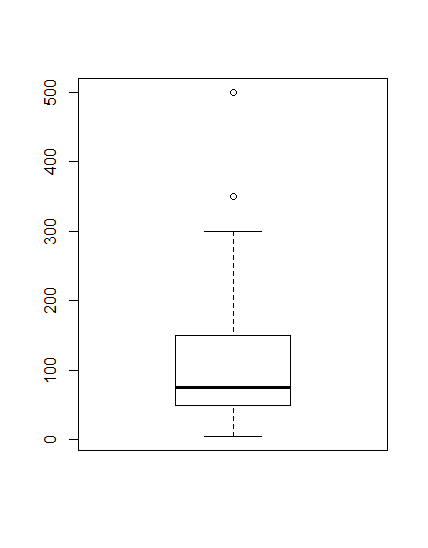
\includegraphics[width=\textwidth,height=\textheight,keepaspectratio]{boxplot_prices.png}
	\caption[Boxplot maximum prijs]{Boxplot over de maximumprijs die een respondent wil betalen voor een GPS-tracker}
	\label{graph:price}
\end{figure}
\newline
Code in R voor het plotten van de boxplot:
\begin{verbatim}
library("readxl")
library(ggplot2)

> prices<-read_excel("C:/Users/IndyV/Desktop/maxPrijs.xlsx")
> prices<-as.numeric(unlist(prices))
> mean<-mean(prices)
> mean
[1] 99.97969
> median<-median(prices)
> median
[1] 75
> prices=data.frame(prices)
> plot <- boxplot(prices)
\end{verbatim}
Een T-test wijst uit dat de gemiddelden op waterbestendigheid (X= 9,61429), accuraatheid (X=8,45714) en gebruiksvriendelijkheid (X=8,05714) significant verschillend zijn, ondanks de relatief kleine steekproef. Hieruit kan geconcludeerd worden dat waterbestendigheid de belangrijkste vereiste is voor respondenten. De proof of concept voldoet aan deze eis.
\newline
\newline
Code in R voor het berekenen van de significantie:
\begin{verbatim}
library("readxl")

> dataset<-read_excel("C:/Users/IndyV/Desktop/dataset.xlsx",col_names=TRUE)
> df<-data.frame(dataset)
> mean_accuraatheid<-mean(df$accuraatheid)
> mean_waterbestendigheid<-mean(df$waterbestendigheid)
> mean_gebruiksvriendelijkheid<-mean(df$ gebruiksvriendelijkheid)
> 
> smallest_mean<-min(mean_accuraatheid,mean_waterbestendigheid,mean_gebruiksvriendelijkheid)
> 
> t.test(df$accuraatheid,mu = smallest_mean)

One Sample t-test

data:  df$accuraatheid
t = 2.0642, df = 69, p-value = 0.04276
alternative hypothesis: true mean is not equal to 8.057143
95 percent confidence interval:
8.070561 8.843725
sample estimates:
mean of x 
8.457143 

> t.test(df$waterbestendigheid,mu = smallest_mean)

One Sample t-test

data:  df$waterbestendigheid
t = 17.422, df = 69, p-value < 2.2e-16
alternative hypothesis: true mean is not equal to 8.057143
95 percent confidence interval:
9.435978 9.792594
sample estimates:
mean of x 
9.614286 

> t.test(df$gebruiksvriendelijkheid,mu = smallest_mean)

One Sample t-test

data:  df$gebruiksvriendelijkheid
t = 0, df = 69, p-value = 1
alternative hypothesis: true mean is not equal to 8.057143
95 percent confidence interval:
7.692046 8.422240
sample estimates:
mean of x 
8.057143 
\end{verbatim}
De batterijduur van de proof of concept voldoet ook aan de eisen van de respondenten, namelijk 24 uur. De batterijduur kan ook verlengd worden indien er gebruik gemaakt wordt van een powerbank.
\newline
Indien de proof of concept op de markt komt, toont 28,6\% van de respondenten zich bereid om deze aanschaffen, ondanks de vrij hoge kostprijs. Een groot deel van de respondenten (54.3\%) twijfelt nog. 
\newline
De proof of concept zou gebruikt worden voor:
\begin{itemize}
	\item watersport = 38,6\&
	\item sneeuwsport = 22,9\%
	\item water- en sneeuwsport = 38,6\%
\end{itemize}
\pagebreak
\section{\IfLanguageName{dutch}{Vergelijking tussen GPS van een gsm en proof of concept}{Difference between the GPS from a phone and the proof of concept}}
Voor de eerste test is er een mobiele applicatie ontwikkeld zodat er gegarandeerd wordt dat de gsm geen gebruik kan maken van extra informatie en/of algoritmen van Google Maps.
\newline
Tijdens de eerste test werden er 2 toestellen gebruikt: de proof of concept en een gsm. De gsm is een Xiaomi Mi 9T (kostprijs 332 euro).
Voor de eerste field test is er op voorhand een route uitgestippeld (zie figuur: \ref{fig:uitgestippelde_route}). Tijdens het wandelen van deze route stuurden de proof of concept (\ref{ch:proof-of-concept}) en de mobiele applicatie (\ref{ch:mobileapp}) tegelijkertijd hun locaties door met een tijdsinterval van telkens drie seconden. (Zie figuur: \ref{fig:field_test_1})
\begin{figure}
	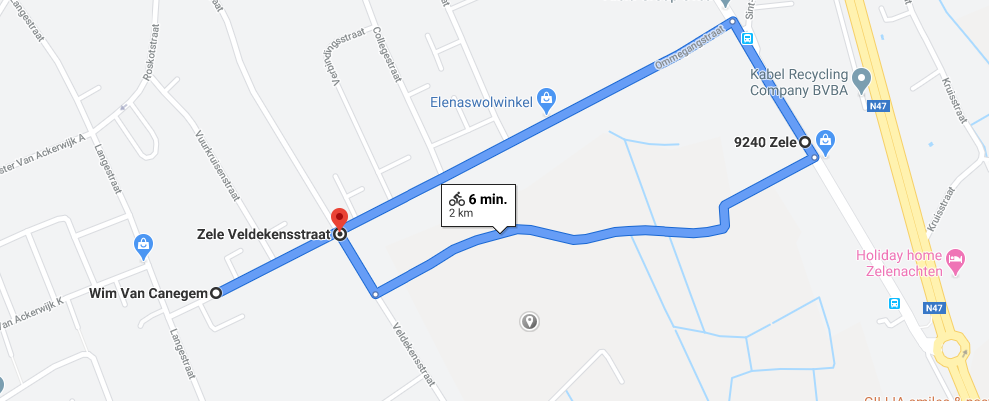
\includegraphics[width=\textwidth,height=\textheight,keepaspectratio]{uitgestippelde_route.png}
	\caption{De uitgestippelde route voor de eerste field test}
	\label{fig:uitgestippelde_route}
\end{figure}
\begin{figure}
	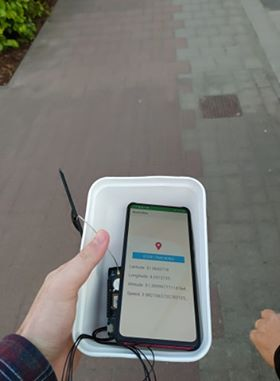
\includegraphics[width=50mm,height=100mm,keepaspectratio]{field_test_1.jpg}
	\caption{Het uitvoeren van de eerste field test}
	\label{fig:field_test_1}
\end{figure}
\newline
\newline
Het resultaat is zeer opmerkelijk. In figuur \ref{fig:field_test_1_resultaat} is het duidelijk dat de proof of concept (blauwe markers) beter scoort dan dan de GPS van een gsm (rode markers). Het is moeilijk om de exacte oorzaak van deze discrepantie in resultaten te achterhalen, omdat de data van de GPS-chip alleen verkrijgbaar zijn voor de fabrikant. De enige data die verkregen kunnen worden van de GPS-chip is de berekende locatie. 
\newline
Het gebruik van Google Maps op een gsm kan een meer accurate locatiebepaling doen in vergelijking met het resultaat van de field test. Dit komt omdat Android en iOS extra informatie gebruiken zoals gsm-masten en wifi signalen (SSIDs). Google Maps maakt ook gebruik van verschillende algoritmen om de locatie te schatten op een straat zodat deze accurater lijken.
\newline
Om de probleemstelling op te lossen, moet een GPS-tracker werken aan de kust en in berggebieden. Ook is de route niet op voorhand geweten, waardoor een gsm zeer slecht zou scoren als GPS-tracker. Google Maps, hetgeen gebruikt wordt door gsm's, bepaalt de locatie immers op basis van straten. In gebieden waar geen of weinig straten zijn, is een exacte locatiebepaling derhalve onmogelijk. De proof of concept lijkt wel een goede oplossing te zijn voor de probleemstelling, omdat het volledig onafhankelijk is van extra informatie en/of algoritmen tijdens het gebruik van Google Maps. 
\newline
Uit de eerste field test kan er dus geconcludeerd worden dat de proof of concept slaagt in zijn opzet.
\begin{figure}
	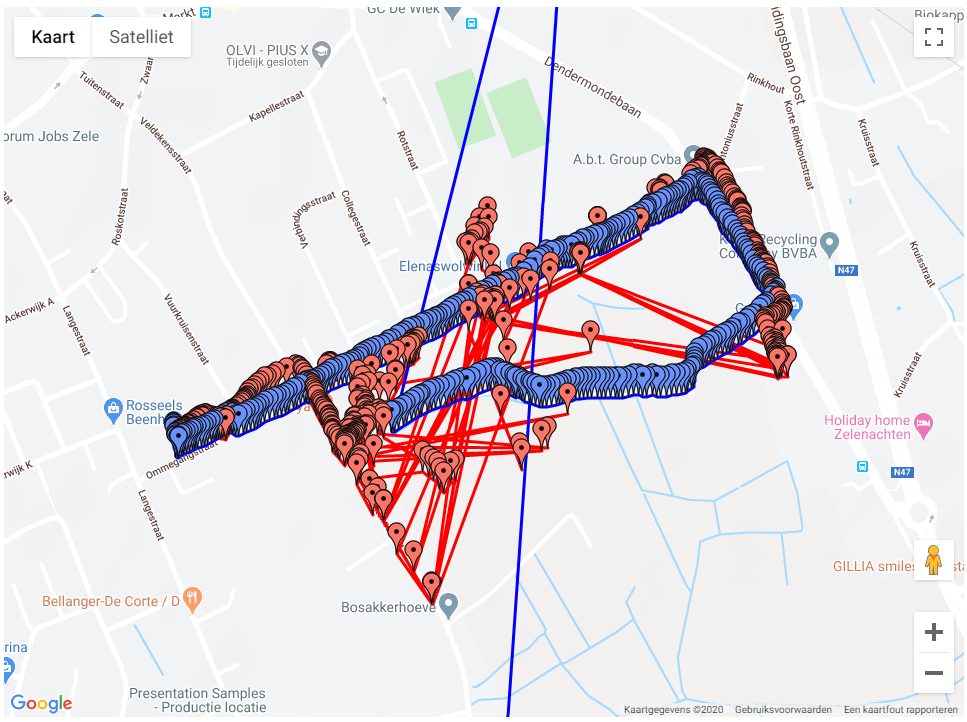
\includegraphics[width=\textwidth,height=\textheight,keepaspectratio]{field_test_1_resultaat.png}
	\caption{Resultaat van de eerste field test}
	\label{fig:field_test_1_resultaat}
\end{figure}
\section{\IfLanguageName{dutch}{Prestaties onder water}{Prestations under water}}
Zoals vermeld in hoofdstuk \ref{ch:stand-van-zaken} kunnen elektromagnetische golven water amper of niet penetreren. Hierdoor leek dit een interessante test.
\newline
De tweede test (zie figuur: \ref{fig:field_test_2}) onderzocht de waterdichtheid van de proof of concept en tot hoe diep de proof of concept kan blijven functioneren. Allereerst blijft de proof of concept functioneren onder het wateroppervlak. Na het openmaken van de behuizing werd er geen water teruggevonden. Om de test uit te voeren is er gebruik gemaakt van een waslijn met markeringen iedere 0,25 meter. 
\newline
Eerst en vooral is er getest geweest tot hoe diep de proof of concept functioneert. De proof of concept kan tot 0,25 meter blijven functioneren. Dit wil zeggen dat, indien het bevestigd wordt aan een surfboard, het in staat is om het surfboard te localiseren. Een surfboard blijft drijven aan het wateroppervlak. Naast de waterbestendigheid moest ook de traceerbaarheid bekeken worden. Om uit te sluiten dat het verzonden GPS-signaal berekend werd boven het wateroppervlak, is de proof of concept op een diepte van 0,25 meter verplaatst rond de hele pier. De verplaatsing van de proof of concept was zichtbaar, waardoor er vastgesteld kan worden dat de proof of concept op een diepte van 0,25 meter perfect functioneert. 
\newline
De resultaten zijn positief, want naast GPS-tracker kan de proof of concept ook als lawinepieper functioneren. De massadichtheid van sneeuw is lager dan die van water, waardoor de proof of concept dieper dan 0,25 meter blijft functioneren. Hoe diep juist, kan niet onderzocht worden wegens de coronapandemie. 
\begin{figure}
	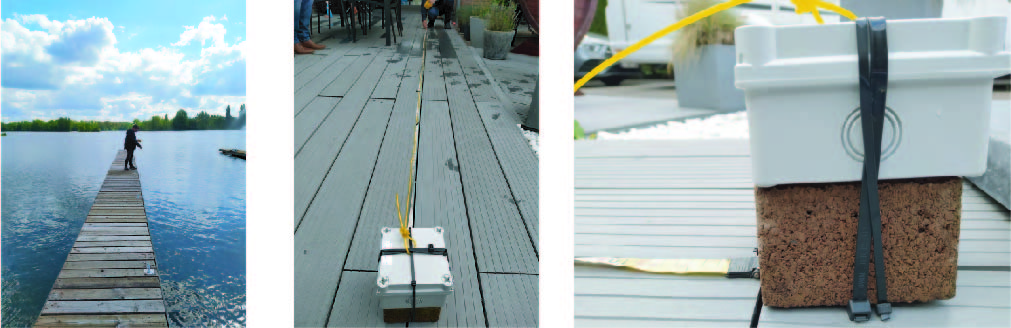
\includegraphics[width=\textwidth,height=\textheight,keepaspectratio]{field_test_2.jpg}
	\caption{Het uitvoeren van de tweede field test}
	\label{fig:field_test_2}
\end{figure}